\section{Multisim: How to Not Get Your Hands Dirty}
\label{lab_multisim}

%\makelabheader %(Space for student name, etc., defined in master.tex)

\bigskip

\begin{enumerate}[wide]

\item Open the program Multisim 14.0 on your computer (under \button{Programs} $\longrightarrow$ \button{Physics Applications}).  
\begin{itemize}
\item Under the \button{Place} menu, select \button{component} to add a component to a circuit.  
\item In the window that opens, under the \button{Group} menu, select \button{Basic}, and under the list of \button{Families} select \button{RESISTOR}.  
\item In the long list to the right, scroll down and click on \button{10k} to select a 10~k$\Omega$ resistor.  Click \button{OK} and then click somewhere on your empty canvas to add the resistor to your circuit diagram.   
\item After placing two resistors on the diagram, right click on each one and select \button{Rotate 90$^\circ$ clockwise} to rotate them so that they look like the figure below.  
\end{itemize}
\begin{center}

\includegraphics{multisim/two_resistors.eps}
\end{center}

\item Continue adding all of the components in the figure below, mimicking the emitter-follower circuit you built in lab~\ref{lab_bjt}. 

\begin{itemize}
\item The capacitor is under the group \button{Basic} in the family \button{CAP\_ELECTROLIT}.  

\item The 2N3904 transistor is under the group \button{Transistors} in the family \button{BJT\_NPN}.

\item The ground symbol is under the group \button{Sources} in the family \button{POWER\_SOURCES}.

\item The power supply VCC is also in the family \button{POWER\_SOURCES}.  To set it to 10 volts instead of the default value of 5, right click and select \button{properties}.

\item The signal generator is under the group \button{Sources} in the family \button{SIGNAL\_VOLTAGE\_ SOURCES}.

\end{itemize}
\begin{center}
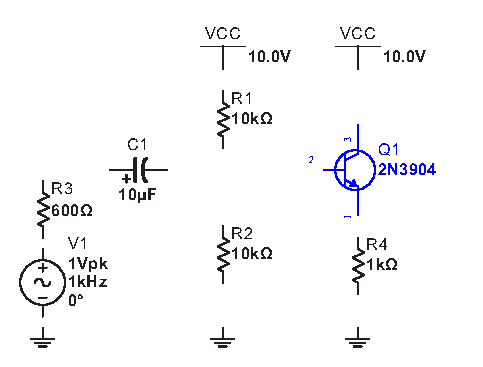
\includegraphics{multisim/more_components.eps}
\index{color_page}
\end{center}

\pagebreak[2]
\item Connect your circuit together.  If you simply click on a terminal of one of the components, Multisim will automatically connect a wire to it.  (Be sure you get a red dot at the four way junction, showing that all four wires are connected there.)  When you finish, your drawing should look like the figure below.  You can always move stuff around after wiring it if you need more room.  Now would be a good time to save your work to your Box account or some other place you can get to later.  Continue to save your work often throughout this lab.
%, and make printouts as needed for your lab notebook (not for this step!).
\begin{center}
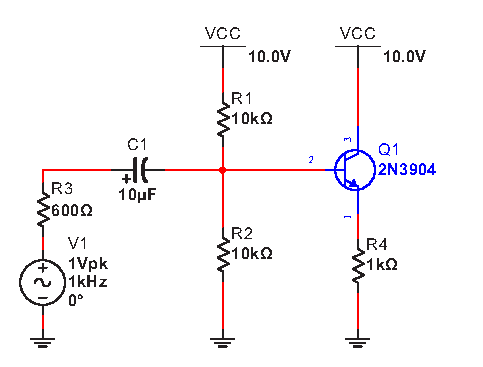
\includegraphics{multisim/wired.eps}
\index{color_page}
\end{center}

\item Making pretty pictures is all well and good, but Multisim also allows you to simulate the behavior of the circuit.  Remove two connecting wires, and add two multimeters, as shown below.  (Multimeters are the top item on the toolbar on the right edge of the screen.)  Double click each one to set them to \button{Amps} and \button{DC}.  With the pop-up windows for each meter still open, choose \button{Simulate} then \button{Run} from the main menu.  What is the apparent value of $h_{FE}$ for this transistor?  You can also start, pause, and stop the simulation using the icons (\raisebox{-0.3ex}{
\includegraphics[height=2ex]{multisim/icons.eps}}) \index{color_page} in the top toolbar.
\begin{center}
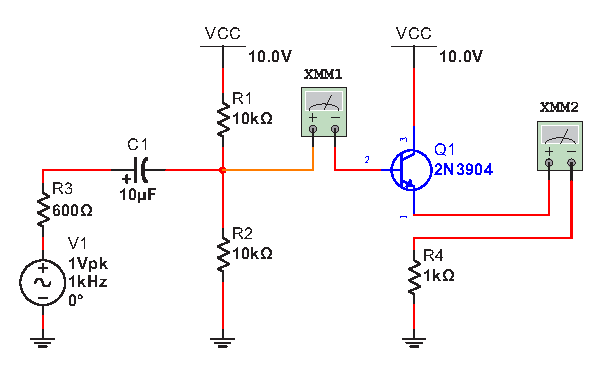
\includegraphics{multisim/multimeters.eps}
\index{color_page}
\end{center}

\item Add an oscilloscope to your circuit to measure the voltage across the load resistor, $R_4$ in the picture above. (The scope is the fourth tiny icon down on the toolbar on the right side of the screen).  The positive lead to input A of the scope will go to your circuit; for the negative lead, you can place another ``ground'' symbol and connect it to your scope.  Before you start simulating, make a prediction of what you should see (both AC and DC parts!).  Is your prediction correct?  Eyeballing values from the graph is fine here; the oscilloscope tool doesn't give you a great way to measure exact values.

\item One of the coolest things Multisim can do is to show you the behavior of your circuit at different frequencies.  Add a ``bode plotter'' to your circuit as shown below.  (It's the sixth icon down on the right-hand toolbar.)  This tool gives you a graph of   as a function of frequency.  Zoom in on the graph by changing the maximum and minimum frequencies, and find the cutoff frequency for this circuit (the $-3$~dB point) using the little slider on the display. \label{part_bode_plotter}
\begin{center}
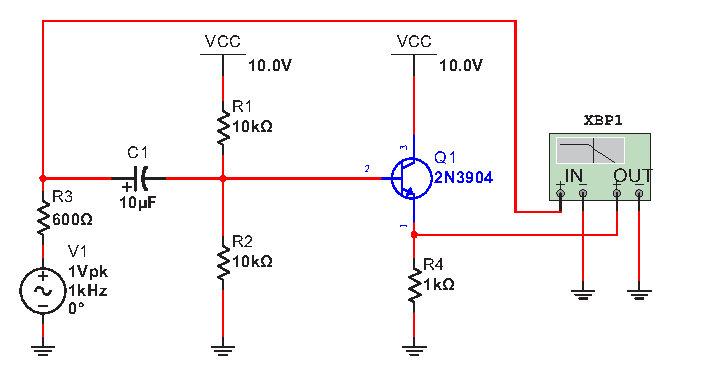
\includegraphics{multisim/bode_plotter.eps}
\index{color_page}
\end{center}

\item As an alternative to the multimeters, Multisim allows you to add a ``measurement probe'' to monitor the voltage and current on a particular wire.  (In the main menu, select \button{Place} $\longrightarrow$ \button{Probe}, or use the little ``V'' and ``A'' icons just to the right of the stop/start buttons.)  Remove the two current meters from your circuit, and replace them with ``voltage and current'' probes.   What additional information do these give you?

\item Use Multisim to design a common emitter amplifier similar to the one we studied in class, but with a gain of  $-20$.  (That is, the AC part of $V_{OUT}$ is 20 times larger than $V_{IN}$, but phase shifted 180 degrees.)  Connect the input of your amplifier to a 0.1~V~AC source through a capacitor, as in the figure in part~\ref{part_bode_plotter} above.  Test your amplifier using Multisim to be certain it has the correct gain.  (Hint: it will be easier if you increase the voltage of the DC supply to 20 volts.)  Make a printout of your circuit showing measurement probe values of the input and output, and include it in your lab notebook. \label{part_emitter_follower}

\item Connect the output of your circuit in part~\ref{part_emitter_follower} to a 200~$\Omega$ load, and watch how everything instantly goes to hell!  :-)  The reason for this is that the load draws lots of current from your amplifier, which throws a monkey wrench into all of the resistor ratios you worked out so carefully.  Use trial and error with Multisim to find out how large the load resistance has to be in order to keep the gain within 95\% or so of what it is with no load. \label{part_problems_with_load}

\item To avoid the problem you ran into in part~\ref{part_problems_with_load}, connect the output of your circuit in part~\ref{part_emitter_follower} to a second amplifier stage with a gain of $G=1$, but with very low output impedance, suitable to drive a 200~$\Omega$ load.  To keep this second stage from drawing too much input current (which would affect the first stage), you may need to use two transistors in the Darlington configuration.  As in lab~\ref{lab_bjt}, you will need to use an additional bypass capacitor on the output to get rid of the DC component of the output. \label{part_common_emitter_and_emitter_follower}


\end{enumerate}

\pagebreak[3]
\textbf{Possible Exam Questions:}

\begin{itemize}

\item Use bipolar junction transistors to design a multi-stage amplifier with a gain $G=100$, capable of a 5~V amplitude output signal.  Use two stages, each with $G=10$, with an additional emitter-follower stage in the middle to correct for any impedance mismatch.  Use additional capacitors and resistors to correctly bias each amplifier stage so that $V_C > V_B > V_E$.

\end{itemize}




